% !Mode:: "TeX::UTF-8"
\documentclass[myposter,portrait]{sciposter}

%% uzitocne package
\usepackage{multicol}
\usepackage{color}
\usepackage{graphicx}

%% znaky s diakritikou
\usepackage[utf8]{inputenc}
\usepackage[T1]{fontenc}
% \usepackage[slovak]{babel} % slovenske delenie slov

%% definicia farieb
% \definecolor{mainCol}{rgb}{0.91,0.82,0.74} % farba pozadia posteru
\definecolor{mainCol}{rgb}{1,1,1} % farba pozadia posteru
\definecolor{sectionCol}{rgb}{0,0,0} % farba nadpisu
\definecolor{textCol}{rgb}{0.2,0,0} % farba hlavneho textu
\definecolor{BoxCol}{rgb}{1,1,0.8} % farba boxu okolo nadpisov

\def\mysection#1{
{\color{sectionCol}\section*{\sc\bfseries #1}}}

\begin{document}
\setlength{\logowidth}{20cm}
\setlength{\titlewidth}{\textwidth}
\addtolength{\titlewidth}{-\logowidth}
\rightlogo[0.9]{fmfilogo-farebne}
\useleftlogofalse

\color{textCol}

\title{Membrane computing}
\author{Michal Kováč\\
        Supervisor: Damas Gruska}
\institute{%
Katedra aplikovanej informatiky,
FMFI UK, Mlynská Dolina, 842~48~Bratislava\\
}
\maketitle

\begin{multicols*}{3}

\mysection{Introduction}
Well established computation models motivated by biology such as neural networks and evolutionary algorithms has already proven that it is worth to be inspired by biology. Other emerging areas are still awaiting for their more significant uses.

One of them is the membrane computing. It is relatively young field of natural computing - in comparison: neural networks have been researched since 1943 and membrane systems since 1998\cite{Paun98}.

\mysection{Membrane structure}

Biological systems usually have hierarchical structure where objects and information flows between regions, what can be interpreted as a computation process.

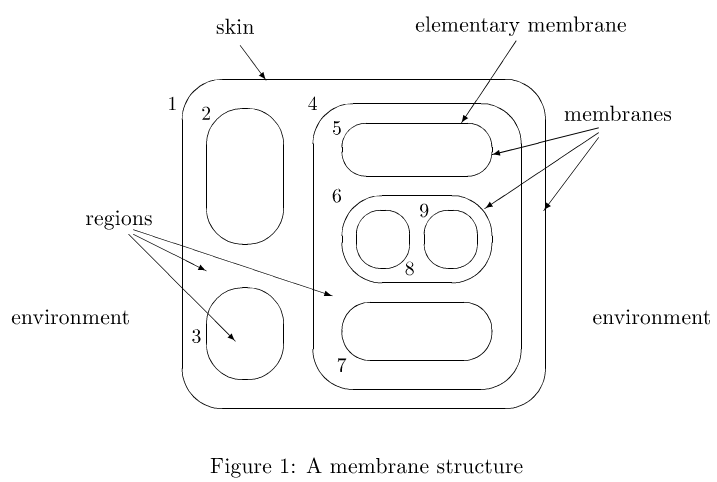
\includegraphics[width=\columnwidth]{membrane_structure}

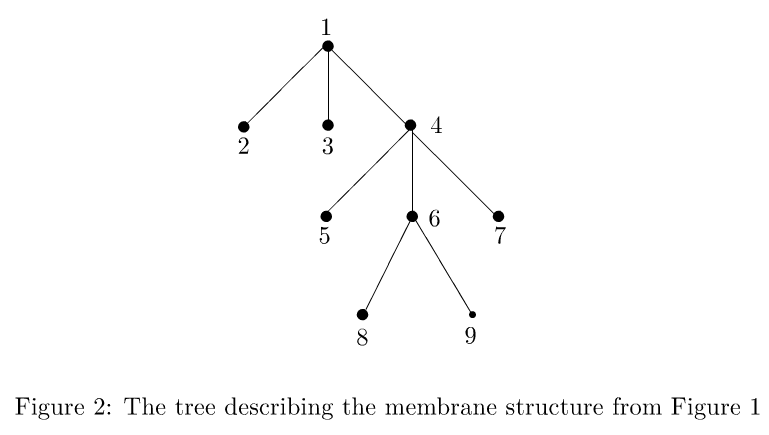
\includegraphics[width=\columnwidth]{membrane_tree}

\mysection{P systems}

Membranes and regions delimited by them has clearly 1:1 correspondence. Each region contains a multiset of objects. These objects can evolve according to evolution rules which are associated with membranes. Evolution rules are applied in a maximally parallel manner - in each step, a maximal multiset of rules is nondeterministically chosen and applied.

This computing device is called P system\footnote{P in P systems stands for surname of it's founder Gheorghe P\u aun.} and is Turing complete.

Next figure demonstrates a computation of a P system for Fibonacci numbers.

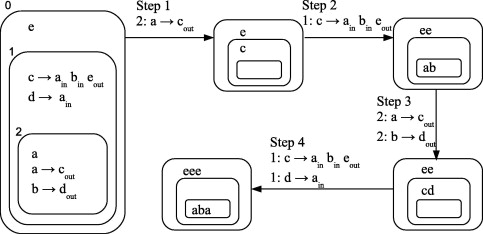
\includegraphics[width=\columnwidth]{p_system_fibonacci}

\mysection{Variants}

Since the first publication in 1998, huge amount of variants has been proposed. Some of them are Turing complete, others are not. Maximal parallelismus is one of the most questioned attribute. P systems in sequential mode are not Turing complete. Various combinations of variants have been studied and some of them have been shown Turing complete also in sequential mode.

\mysection{Inhibitors}

Rewrite rules may contain inhibitors; their presence in the region prevents the application of the rule. We show that sequential P systems with inhibitors are Turing complete.


     By introducing the product topology on  $R^{m \times m} \times
R^{n \times n}$  with the induced inner product
\begin{equation}
\langle (A_{1},B_{1}), (A_{2},B_{2})\rangle := \langle A_{1},A_{2}\rangle 
+ \langle B_{1},B_{2}\rangle,\label{eq2.10}
\end{equation}
we calculate the Fr\'{e}chet derivative of  $F$  as follows:
\begin{eqnarray}
 F'(U,V)(H,K) &=& \langle R(U,V),H\Sigma V^{T} + U\Sigma K^{T}\nonumber\\
             && - P(H\Sigma V^{T} + U\Sigma K^{T})\rangle \nonumber \\
         &=& \langle R(U,V),H\Sigma V^{T} + U\Sigma K^{T}\rangle\nonumber \\
&=& \langle R(U,V)V\Sigma^{T},H\rangle + \nonumber\\
  &&    \langle \Sigma^{T}U^{T}R(U,V),K^{T}\rangle.    \label{eq2.11}
\end{eqnarray}

In the middle line of (\ref{eq2.11}) we have used the fact that the range of
$R$ is always perpendicular to the range of $P$.  The gradient $\nabla F$  of
$F$, therefore,  may be interpreted as the
pair of matrices:
\begin{eqnarray}
 \nabla F(U,V) &=& (R(U,V)V\Sigma^{T},R(U,V)^{T}U\Sigma )\nonumber\\
 && \in R^{m \times m} \times R^{n \times n}.   \label{eq2.12}
\end{eqnarray}

Thus, the vector field
\begin{equation}
\frac{d(U,V)}{dt} = -g(U,V) 	\label{eq2.15}
\end{equation}
defines a steepest descent flow on the manifold  ${\cal O} (m) \times
{\cal O} (n)$ for the objective function  $F(U,V)$.

\columnbreak 

\mysection{Numerical experiments} 

We conducted numerical experiments 
in computing inexact Newton steps for discretizations of a  
{\em modified Bratu problem}, given by  
\begin{eqnarray} 
{\displaystyle \Delta w + c e^w + d{ {\partial w}\over{\partial x} } } 
&=&{\displaystyle f \quad {\rm in}\ D, }\nonumber\\[-1.5ex]
\label{bratu} \\[-1.5ex]
{\displaystyle w }&=&{\displaystyle 0 \quad {\rm on}\ \partial D , } \nonumber
\end{eqnarray} 
where $c$ and $d$ are constants. The actual Bratu problem has $d=0$ and  
$f \equiv0$.

\def\gmres{{GMRES}} 
\def\gmresm{{\rm GMRES($m$)}} 

In our experiments, we took $D = [0,1]\times[0,1]$, $f \equiv0$, 
$c=d=10$, and discretized (\ref{bratu}) using the usual second-order 
centered differences over a $100\times100$ mesh of equally 
spaced points in $D$. In \gmres($m$), we took $m=10$ and used fast  
Poisson right preconditioning as before.

\bigskip 
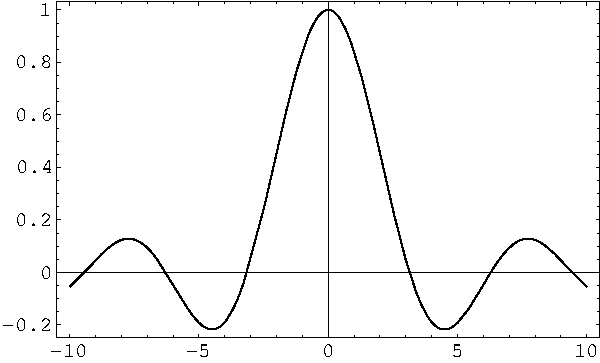
\includegraphics[width=\columnwidth]{fig}
\caption{Graph of the function $\sin(x)/x$.} 
 

%% zoznam literatury
\bibliographystyle{apalike}
\bibliography{references}

\end{multicols*}
\end{document}

